\documentclass[11pt]{article}
\usepackage{common}
\usepackage{listings}
\usepackage{hyperref}
\usepackage{graphicx}
\usepackage{subcaption}
\graphicspath{ {images/} }
\lstset{breaklines=true}

\title{A Comparison of Deep Q-Learning algorithms with Atari}
\author{Michelle Chiang, Daniel Seong, Andrew Fai \\ \href{https://github.com/afai/cs182-project/tree/master/}{https://github.com/afai/cs182-project/tree/master/}}
\begin{document}
\maketitle{}


\section{Introduction}

The combination of deep neural networks and reinforcement learning has received a great deal of attention recently due to remarkable breakthroughs in teaching computers to perform tasks with human or even super-human capabilities. When applied to Atari, the games pose a unique challenge: a shared observation and action space, but different goals, rules, and reward structures. The purpose of our project is to create a general neural network structure that can train effective agents for various Atari games using variants of the Q-Learning algorithm. We first adopted Google DeepMind's original algorithm and developed a convolutional neural network that uses deep Q-learning to train agents \cite{mnih}. Then, we improved the training time and performance of the model by implementing algorithm modifications such as target networks, asynchronous multithreading, and N-step Q-learning, as well as input variations between screen images and RAM states. Finally, we tested our models by comparing performance across three Atari games: Breakout, Atlantis, and BeamRider. We thus produced a generalized model that is equipped to handle the different mechanics and goals of these Atari games without any prior knowledge.

\section{Background and Related Work}

Convolutional neural networks (CNNs) made their debut in 2012, when Alex Krizhevsky utilized them in his submission to the ImageNet competition. More accurate than any previous image classification models had been, CNNs passed images through convolutional layers with ReLU activations and a fully connected layer at the end, which outputted a vector of class probabilities. The power of this model was a convolutional layer's ability to capture local connectivity, allowing a series of them to reduce the set of pixels in an image into identifiable objects. At the time, games still used traditional reinforcement learning that relied heavily on human-created feature representations; as such, there were no applications that could be generalized to a wide range of environments.

DeepMind Technologies changed this in 2013 by publishing "Playing Atari with Deep Reinforcement learning." The authors successfully combined reinforcement learning and deep learning to create a CNN that, when applied to seven Atari 2600 games, outperformed "all previous approaches on six" and "surpassed a human expert on three" \cite{mnih}. The researchers surmised that the essential information to learn to play the game well, such as agent behavior and action consequences, was encoded within screen images, allowing the model to generalize to a wide range of games. Despite the inherent differences between reinforcement learning, which learned from reward signals that could be sparse or delayed, and deep learning, which required labeled training data, the DeepMind researchers created a variant of the Q-learning algorithm, which used stochastic gradient descent to train a CNN that received screen images and returned a vector of Q-values, in which each element represented a legal action \cite{mnih}. Once trained, this CNN could be used to compute the best action given the current observation of the screen, allowing it to effectively play Atari games.

\section{Problem Specification}

In our original proposal, we planned on investigating classical search as well. However, we quickly found that this was not feasible for two reasons: the state space was far too large, with size $128^{256}$ RAM and an even greater size for screen images; and the Arcade Learning Environment that OpenAI Gym used for Atari did not support look-ahead very well. As such, it became apparent that deep Q-Learning was the superior approach if we wanted to train successful agents.

Our focus was not on the CNN structure itself, but rather on the comparison of deep Q-Learning algorithms. We implemented three: Deep Q-Learning Networks (DQN) with experience replay, Asynchronous DQN, and Asynchronous N-Step Q-Learning algorithms. Finally, we compared these algorithms across three different games: Breakout, BeamRider, and Atlantis.

\section{Approach}

We began by creating two CNNs, one for screen images and the other for RAM. They screen image CNN had structure,
\begin{center}
\begin{tabular}{ c c c c c }
 Layer          & Kernel    & Stride    & Filters   & Activation    \\ \hline
 Convolution 1  & $(8,8)$   & 4         & 8         & ReLU          \\
 Convolution 2  & $(4,4)$   & 2         & 16        & ReLU          \\
 Convolution 3  & $(3,3)$   & 1         & 32        & ReLU          \\ \hline\hline
 Layer          & Input length          & Output Length     &  & Activation    \\ \hline
 Linear 1       & size(Convolution 3)   & 256               &  & ReLU          \\
 Linear 2       & 256                   & size(Action Space)&  & None
\end{tabular}
\end{center}
and the RAM CNN had structure
\begin{center}
\begin{tabular}{ c c c c c }
 Layer          & Kernel    & Stride    & Filters   & Activation    \\ \hline
 Convolution 1  & $1$       & 1         & 8         & ReLU, Dropout \\
 Convolution 2  & $1$       & 1         & 16        & ReLU, Dropout \\ \hline\hline
 Layer          & Input length          & Output Length     & & Activation    \\ \hline
 Linear 1       & size(Convolution 2)   & size(Action Space)& & None
\end{tabular}
\end{center}
Our CNN for screen images was based very similar to DeepMind's, and we based our CNN for RAM off of this; the difference was that we used Kernel size 1 so that no local connectivity assumptions are made about RAM, and we used a Dropout activations for the regularization. In general, we used ReLU activations for each layer such that the gradient of loss with respect to the model parameters is non-linear.

Once we created our networks, we implemented the three algorithms. The first, DQN with experience replay, couples the Q-learning algorithm we learned in class with experience replay - a technique where, for a specified number episodes, the algorithm selects an action using an epsilon-greedy strategy, carries out the action, and stores the observed terminality, transition, and reward in memory as an experience. Then, the algorithm samples a batch of these experiences and uses these transitions to train the model. The motivation for experience replay is so that the agent does not "forget" non-recent experiences, since recent states are very likely to be similar.

The second algorithm, Asynchronous DQN, replaces experience replay with asynchronous training. Instead of storing transitions in memory and sampling them later on, it runs Q-learning on multiple threads at once (the exact number depends on how many available cores the system has). Each thread interacts with its own environment and periodically updates a global network using the Q-learning loss.

The final algorithm is asynchronous N-step Q-learning. This algorithm is similar to the asynchronous Q-learning, but instead of updating the single most recent Q-value, it updates the N previous Q-values. We record the previous rewards, states, and actions and add a simple for loop after termination to update N previous Q-values.

All three algorithms utilize stochastic gradient descent and a function of the difference between the left and right sides of the Bellman equation as loss during backpropagation. The function we chose was Huber Loss, which is less sensitive to outliers. When working with image inputs, we apply a pre-processing step that converts each image to gray-scale and down-samples its size in order to reduce computational demand. Finally, the inputs of the model are adjusted to not be the most recent screen observation, but rather a stack of the most recent 4, in order to assist the CNN in learning the movement of objects over time and ultimately helping with credit assignment.

Pseudo-code for DQN with Experience Replay\cite{mnih}, Asynchronous DQN\cite{mnihAsync}, and Asynchronous N-step Q-learning algorithms \cite{mnihAsync} can be found in Algorithm 1, 2, and 3, respectively: \\
\begin{figure}[H]
    % \centering
    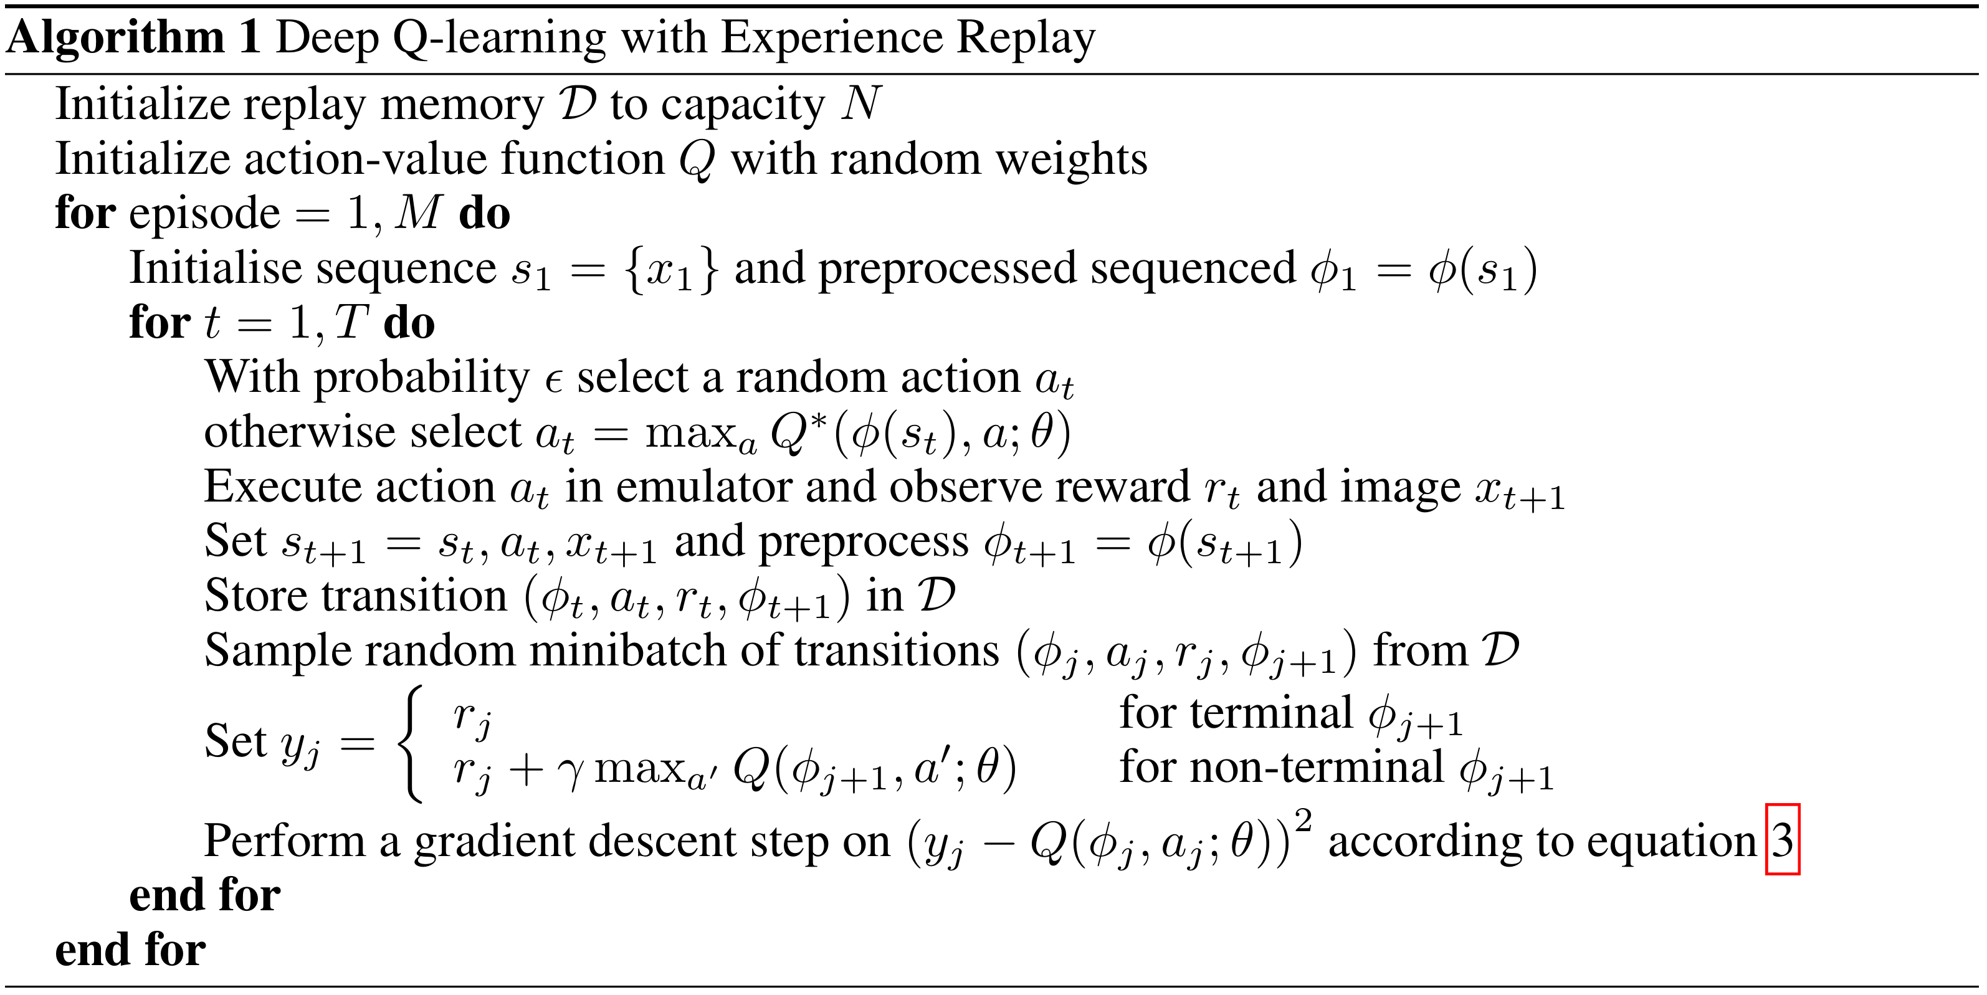
\includegraphics[scale=0.4]{dqn}
\end{figure}
\begin{figure}[H]
    % \centering
    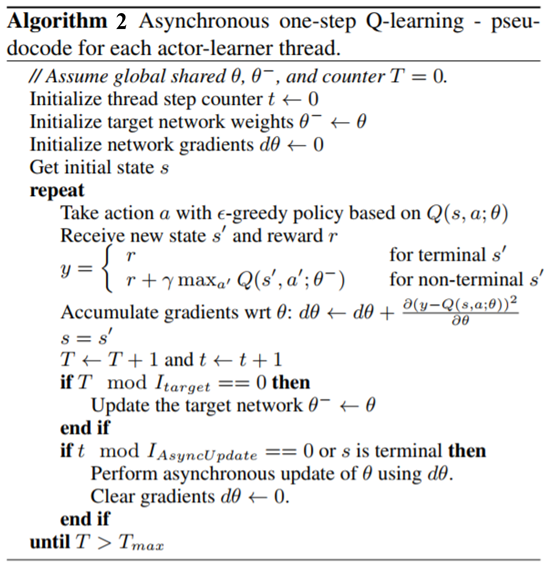
\includegraphics[scale=1.1]{asynchronous}
    \label{fig:my_label}
\end{figure}
\begin{figure}[H]
    % \centering
    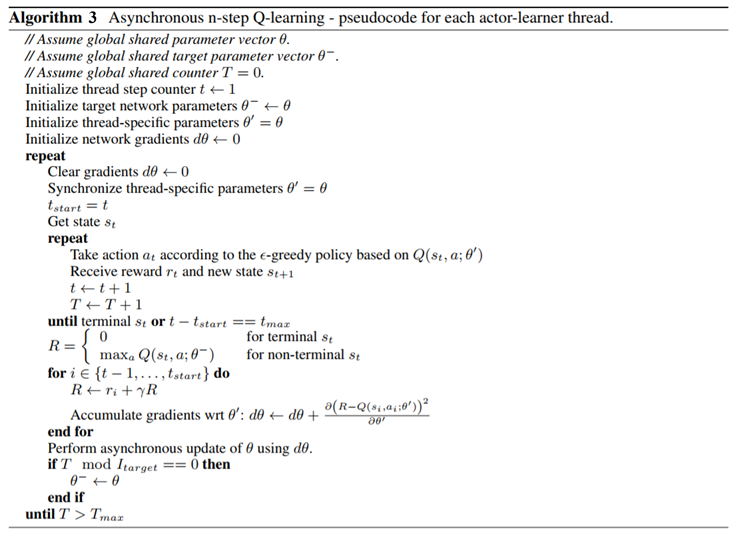
\includegraphics[scale=1.3]{nstep}
\end{figure} \newpage

\section{Experiments}

When choosing which Atari games to focus on, we prioritized breadth of difficulty in order to test our algorithm's performance. For individual rewards, Atlantis requires single actions, Breakout requires a sequence of motions, and BeamRider requires both. Using the OpenAI Gym platform to run the Atari games, we tested all algorithms for all games using RAM inputs; then, we tested Asynchronous N-Step Q-Learning for all games using screen inputs.
 
Because time was our limited resource (DeepMind trained its original model for 10-12 days on computers much more powerful than ours), we set the number of episodes for training runs such that each run was in the range of 60-100 minutes. For the asynchronous methods, we used 4 threads. Our discount rates was 0.99, such that Q-values could theoretically converge without fabricating non-existent actual discounts. Under our epsilon-greedy approach, epsilon started at 1.0 and linearly decreased to 0.1 over the first 70\% of episodes before plateauing. We saved the training scores and smoothed them with a moving average of 100 episodes.
 
Once we trained all of our models, we tested them by running 100 episodes and recording mean and standard deviation of each; we also tested using a random agent for each game.

\subsection{Results}

The test results were as follows. Note that the Episodes and Time columns represent training, whereas the $\mu\pm\sigma$ columns represents the 100-episode tests after training.
\begin{center}
\begin{tabular}{ l | c | c | r | r }
 Atlantis                       & Input     & $\mu\pm\sigma$    & Episodes  & Time  \\ \hline
 Random                         &           & $19434 \pm 7218$  &           &       \\
 DQN with Experience Replay     & RAM       & $33246 \pm 9615$  & 500       & 5087  \\
 Asynchronous DQN               & RAM       & $36810 \pm 10546$ & 10000     & 4388  \\
 Asynchronous N-Step Q-Learning & RAM       & $7895 \pm 3625$   & 10000     & 4000  \\
 Asynchronous N-Step Q-Learning & Screen    & $8059 \pm 2714$   & 4000      & 4283  \\ \hline\hline
 BeamRider                      &           &                   &           &       \\ \hline
 Random                         &           & $345 \pm 148$     &           &       \\
 DQN with Experience Replay     & RAM       & $515 \pm 166$     & 600       & 5183  \\
 Asynchronous DQN               & RAM       & $248 \pm 74$      & 12000     & 5981 \\
 Asynchronous N-Step Q-Learning & RAM       & $644 \pm 190$     & 15000     & 6825  \\
 Asynchronous N-Step Q-Learning & Screen    & $813 \pm 233$     & 4000      & 6033  \\ \hline\hline
 Breakout                       &           &                   &           &       \\ \hline
 Random                         &           & $1.26 \pm 1.28$   &           &       \\
 DQN with Experience Replay     & RAM       & $1.96 \pm 1.22$   & 2500      & 4349  \\
 Asynchronous DQN               & RAM       & $2.42 \pm 2.19$   & 50000     & 3592  \\
 Asynchronous N-Step Q-Learning & RAM       & $3.62 \pm 2.90$   & 50000     & 4820  \\
 Asynchronous N-Step Q-Learning & Screen    & $8.62 \pm 3.12$   & 15000     & 6818
\end{tabular}
\end{center}

\noindent As a proof of concept, we trained a model using Asynchronous N-Step Q-Learning on Breakout for screen images for 50000 episodes. The test results were $20.38 \pm 9.00$. \\

\noindent The plot of training scores over time are below:
\begin{figure}[H]
    \centering
    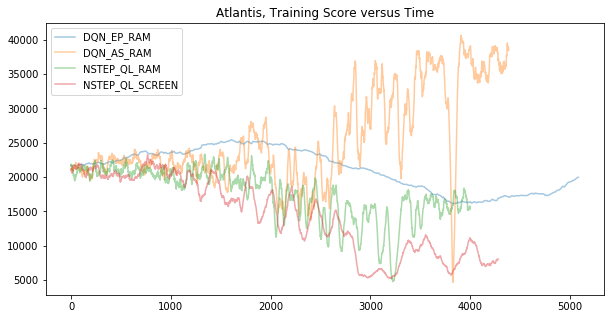
\includegraphics[scale=0.6]{atlplot}
\end{figure}
\begin{figure}[H]
    \centering
    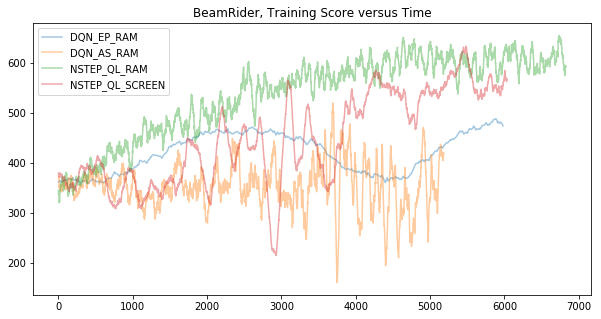
\includegraphics[scale=0.6]{bmrplot}
    \label{fig:my_label}
\end{figure}
\begin{figure}[H]
    \centering
    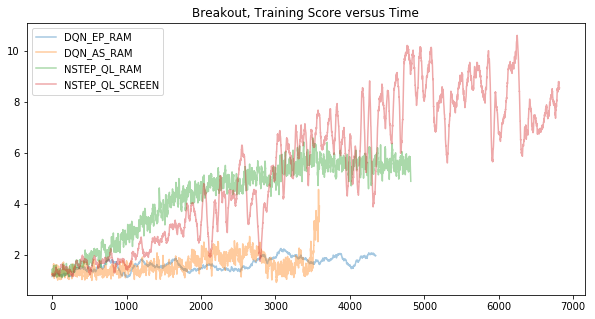
\includegraphics[scale=0.6]{brkplot}
\end{figure}



\section{Discussion}

Across all three games, DQN with experience replay is clearly suboptimal. It takes longer to perform because it randomly samples very often and does not take advantage of multiprocessing, thus learning less over time than the other two algorithms. The original DeepMind model utilized experience replay to break the issue of highly similar successive states that could drive the network to a local minimum \cite{minh}. However, running multiple agents in parallel takes advantage of the computer's full resources while also solving the issue of recency bias, since the model updates are not dominated by a single recent experience; at any given time, all agents will likely be seeing different states.

For Breakout and BeamRider, Asynchronous N-Step Q-Learning trains the most quickly with respect to time, with RAM appearing to be a little more stable overall. In testing, however, the screen images outperform RAM inputs across all three games when using this algorithm. On the other hand, for Atlantis it performs the worst, while Asynchronous DQN performs the best. This failure for Asynchronous N-Step Q-Learning to outperform even DQN with experience replay is perhaps the most surprising result, and it remains a question whether more training time would rectify this.

Our assumption for why Asynchronous N-Step Q-Learning outperformed the other two algorithms for BeamRider and Breakout is that true rewards are backpropogated more quickly; in the other two algorithms, only the current state and next state are used for optimization, whereas for N-Steps, N states are used.

The random agent was a very different benchmark across games. Since Atlantis requires firing bullets at planes that are flying by - i.e., singular actions that yield rewards - the random agent actually performed quite well, beating both inputs on Asynchronous N-Step Q-Learning. For BeamRider and especially Breakout, this was not the case, since rewards required a sequence of movements towards a correct location in order to achieve rewards, making the random agent less likely to do so.

Comparing RAM and screen inputs, we see that the networks learn much more quickly per episode when using the screen, but over time the results are very similar, since we can run about 3-4 times more episodes using RAM in a fixed training duration. In practice, there is a trade-off between RAM input, which is memory efficient, and screen image input, which takes fuller advantage of CNN's ability to localize objects. Even though RAM had smoother training results, testing showed that screen inputs yielded higher success.

Overall, the algorithms showcased the power of convolutional neural networks combined with reinforcement learning: without any human input as to the identity or rules of a game, our agent was able to consistently improve its score during training, overcoming inherent differences in games that presented challenges. Additionally, by implementing asynchronous and utilizing multiple actors, our agent was able to tackle these challenges and consistently improve over training, ultimately achieving decent performance with only around 20 hours of training.

In future work, we could test our algorithm over a wider range of the Atari games provided by OpenAI Gym with higher numbers of iterations, computational power allowing. Furthermore, we could further explore the effects of our optimizations, such as by testing performance as a function of $n$ asynchronous learners.

\appendix

\section{System Description}

 Appendix 1 – A clear description of how to use your system and how to generate the output you discussed in the write-up. \emph{The teaching staff must be able to run your system.}
 \subsection*{Windows Ubuntu Bash shell}
 \subsubsection*{List of components}
 \begin{itemize}
  \item Anaconda 3
  \item Pytorch 
  \item Several additional packages: 
  \begin{itemize}
      \item Cross-platform, open source, build tool cmak
      \item Free and open compression library, zlib1g-dev 
      \item X Window system development libraries xorg-dev
      \item GTK+ (GIMP Toolkit) libgtk2.0-0
      \item Python 2D plotting library python-matplotlib
      \item Wrapper generator swig
      \item Python OpenGL Binding python-opengl
  \end{itemize}
\end{itemize}

 \subsubsection*{Install Anaconda 3}
 \begin{lstlisting}[language=bash]
    $ wget http://tex.stackexchange.com
    $ bash Anaconda3-4.2.0-Linux-x86_64.sh
 \end{lstlisting}
 \subsubsection*{Install supporting packages}
 \begin{lstlisting}[language=bash]
    $ sudo apt-get install cmake zlib1g-dev xorg-dev libgtk2.0-0 python-matplotlib swig python-opengl
    $ source ~/.bashrc
 \end{lstlisting} 
 \subsubsection*{Create conda environment for gym}
  \begin{lstlisting}[language=bash]
    $ conda create --name gym python=3.5
    $ source activate gym
 \end{lstlisting} 
 \subsubsection*{Install OpenAI gym}
 \begin{lstlisting}[language=bash]
    (gym) $ git clone https://github.com/openai/gym
    (gym) $ cd gym
    (gym) $ pip install -e .[all]
 \end{lstlisting} 
 \subsubsection*{Install matplotlib}
 \begin{lstlisting}[language=bash]
    (gym) $ pip install matplotlib
 \end{lstlisting}
 \subsubsection*{Install X Windows Libraries}
 First, download Xming installer from \url{https://sourceforge.net/projects/xming/files/latest/download}. Then let your system know about this display:
 \begin{lstlisting}[language=bash]
    (gym) $ export DISPLAY=:0
 \end{lstlisting}     
 \subsubsection*{Install Pytorch}
 \begin{lstlisting}[language=bash]
    (gym) $ conda install pytorch torchvision -c pytorch
 \end{lstlisting}     
 \subsection*{Mac}
  \begin{lstlisting}[language=bash]
    $ bash <(curl -Ls https://raw.githubusercontent.com/AISafetyClub/scripts/master/gym_installer.sh)
  \end{lstlisting} 
  
\subsection*{Running the Program}
In order to train the agent, set the relevant parameters in `train.py` and run `python train.py`, which also automatically generates plots tracking the agent's performance over each iteration. In order to see the agent in action, run `rungym.py`.

\section{Group Makeup}

Appendix 2 
\begin{itemize}
    \item Andrew - research, implementation and testing of algorithms
    \item Daniel - testing and analysis of algorithms
    \item Michelle - testing and analysis of algorithms
\end{itemize}

\bibliographystyle{plain} 
\bibliography{final-writeup}

\end{document}
